\section{Results}
    The frequency we read from the signal generator is $f=35000\pm 1$Hz. The temperature is $24\pm1\SI{}{\degreeCelsius}$.
\subsection{Measurements for resonance method}
    The measurements are shown in Table \ref{data_res} with the calculation for $L_{10+i}-L_i$.
    \begin{table}[h] \small
        \centering
        \begin{tabular}{|c|c|c|c|c|c|}
        \hline
            \multicolumn{2}{|c|}{$L_i[\e{-3}m]\pm[0.01\e{-3}m]$} & 
            \multicolumn{2}{|c|}{$L_i[\e{-3}m]\pm[0.01\e{-3}m]$} &
            \multicolumn{2}{|c|}{$L_{10+i}-L_i[\e{-3}m]$}\\\hline
            1 & 9.90 & 11 & 60.08 & 1 & 50.18 \\\hline
            2 & 14.92 & 12 & 65.08 & 2 & 50.16 \\\hline
            3 & 19.97 & 13 & 70.06 & 3 & 50.09 \\\hline
            4 & 25.02 & 14 & 75.02 & 4 & 50.00 \\\hline
            5 & 30.03 & 15 & 80.25 & 5 & 50.22 \\\hline
            6 & 35.06 & 16 & 85.24 & 6 & 50.18 \\\hline
            7 & 40.03 & 17 & 90.24 & 7 & 50.21 \\\hline
            8 & 45.08 & 18 & 95.22 & 8 & 50.14 \\\hline
            9 & 49.95 & 19 & 100.13 & 9 & 50.18 \\\hline
            10 & 55.01 & 20 & 105.24 & 10 & 50.23 \\\hline
        \end{tabular}
        \caption{Data for the resonance method}\label{data_res}
    \end{table}
    The average value of $\Delta L$ is calculated  based on the results presented in Table \ref{data_res} as
    \[
        \overline{\Delta L}=\frac{1}{10}\sum_{i=1}^{10}\Delta L_i=(50.16\pm 0.05)\e{-3}m,\quad u_{r,\Delta L}=0.10\%.
    \]
    Hence, the wavelength $\lambda$ can be calculated as
    \[
        \lambda=\frac{2\Delta L}{n}=\frac{2\times50.16\e{-3}}{10}=(10.03\pm0.01)\e{-3}m,\quad u_{r,\lambda}=0.10\%.
    \]
    The speed of sound in air $v$ is
    \[
        v=351.05\pm0.4 m/s,\quad u_{r,v}=0.10\%.
    \]

\subsection{Measurements for phase comparison method}
    The measurements are shown in Table \ref{data_pha} with the calculation for $L_{6+i}-L_i$.
    \begin{table}[h] \small
        \centering
        \begin{tabular}{|c|c|c|c|c|c|}
        \hline
            \multicolumn{2}{|c|}{$L_i[\e{-3}m]\pm[0.01\e{-3}m]$} & 
            \multicolumn{2}{|c|}{$L_i[\e{-3}m]\pm[0.01\e{-3}m]$} &
            \multicolumn{2}{|c|}{$L_{6+i}-L_i[\e{-3}m]$}\\\hline
            1 & 54.00 & 7 & 113.41 & 1 & 59.41 \\\hline
            2 & 64.06 & 8 & 122.04 & 2 & 57.98 \\\hline
            3 & 72.97 & 9 & 131.76 & 3 & 58.79 \\\hline
            4 & 81.02 & 10 & 141.83 & 4 & 60.81 \\\hline
            5 & 91.17 & 11 & 153.65 & 5 & 62.46 \\\hline
            6 & 103.49 & 12 & 163.08 & 6 & 59.59 \\\hline
        \end{tabular}
        \caption{Data for the phase comparison method}\label{data_pha}
    \end{table}
    The average value of $\Delta L$ is calculated  based on the results presented in Table \ref{data_res} as
    \[
        \overline{\Delta L}=\frac{1}{6}\sum_{i=1}^{6}\Delta L_i=(59.84\pm 1.7)\e{-3}m,\quad u_{r,\Delta L}=3\%.
    \]
    Hence, the wavelength $\lambda$ can be calculated as
    \[
        \lambda=\frac{\Delta L}{n}=\frac{\times59.84\e{-3}}{6}=(9.973\pm0.3)\e{-3}m,\quad u_{r,\lambda}=3\%.
    \]
    The speed of sound in air $v$ is
    \[
        v=348.95\pm10 m/s,\quad u_{r,v}=3\%.
    \]
\subsection{Measurements for time difference method (liquid)}
    We obtain the speed of sound in water from Table \ref{data_tim} by linear fitting (See Figure \ref{lt}).
    \begin{table}[H] \small
        \centering
        \begin{tabular}{|c|c|c|c|c|}
        \hline
            & $t_i[\e{-6}s]$ & $u_{t_i}[\e{-6}s]$ & $L_i[\e{-3}m]$ & $u_{L_i}[\e{-3}m]$\\\hline
            1 & 159.6 & 0.2 & 230.00 & 0.01\\\hline
            2 & 154.4 & 0.2 & 220.00 & 0.01\\\hline
            3 & 148.2 & 0.2 & 210.00 & 0.01\\\hline
            4 & 141.8 & 0.2 & 200.00 & 0.01\\\hline
            5 & 134.0 & 0.2 & 190.00 & 0.01\\\hline
            6 & 128.0 & 0.2 & 180.00 & 0.01\\\hline
            7 & 121.4 & 0.2 & 170.00 & 0.01\\\hline
            8 & 114.4 & 0.2 & 160.00 & 0.01\\\hline
            9 & 108.0 & 0.2 & 150.00 & 0.01\\\hline
            10 & 101.6 & 0.2 & 140.00 & 0.01\\\hline
            11 & 94.8 & 0.2 & 130.00 & 0.01\\\hline
            12 & 87.8 & 0.2 & 120.00 & 0.01\\\hline
        \end{tabular}
        \caption{Data for Figure \ref{lt}}\label{data_tim}
    \end{table}
    \begin{figure}[H]
        \centering
        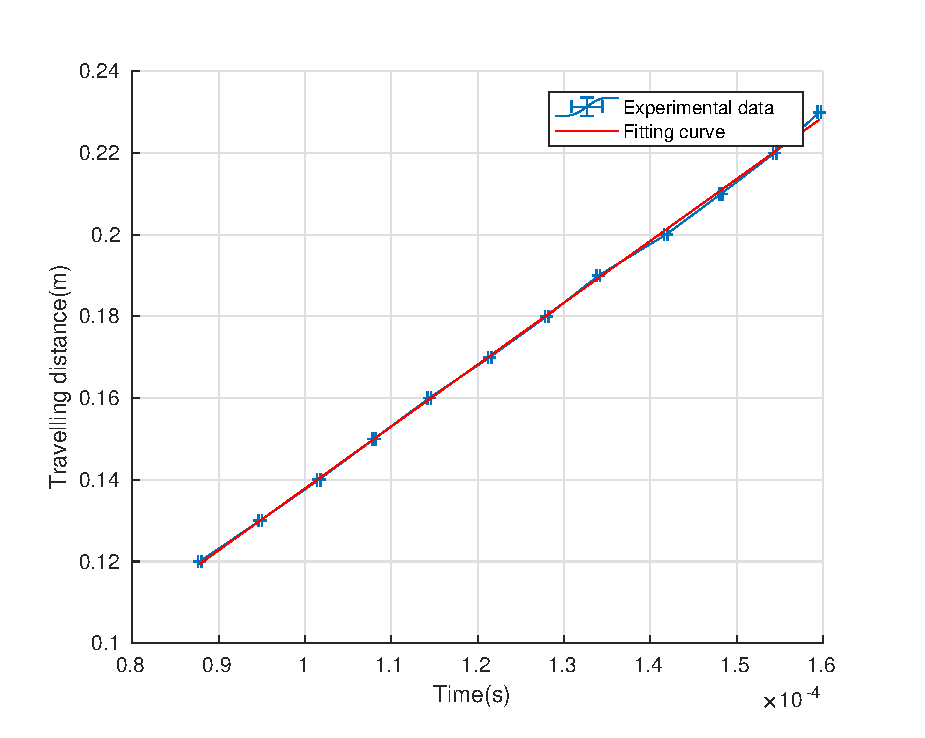
\includegraphics[height=10cm]{images/lt.eps}
        \caption{Fitting curve for $L\ vs.\ t$. (The errorbar is relatively \textbf{small})}\label{lt}
    \end{figure}
    \begin{figure}[H]
        \centering
        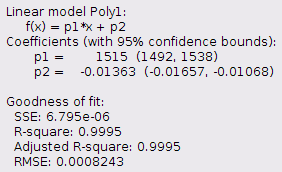
\includegraphics[height=6cm]{images/ltinfo.png}
        \caption{Information for Fitting curve in Figure \ref{lt}}\label{ltinfo}
    \end{figure}

    From the data processing of Matalb we know about the slope that 
    \[
        v_{water}=1515\pm20m/s.
    \]